\ifdefined\beamerclass
\else
  \def\beamerclass{beamer}
\fi

\ifdefined\articlemode
	\documentclass[]{article}
	\usepackage[a4paper,margin=2cm]{geometry}
	\usepackage[envcountsect]{beamerarticle}
	\usepackage{parskip}
	\usepackage[hidelinks]{hyperref}
\else
	 \documentclass[\beamerclass,ignorenonframetext]{beamer}
\fi

\usepackage{pgfpages}
\mode<handout>{
	% \setbeamercolor{background canvas}{bg=black!20}
	\pgfpagesuselayout{2 on 1}[a4paper,border shrink=5mm]
}

\usepackage{lmodern}
\usepackage{listings}
\usepackage{amsmath}
\usepackage{bm}
\usepackage{textpos} % package for the positioning

\usepackage{pgf, tikz}
\usepackage{pgfplots}
\usetikzlibrary{arrows, automata}

\usetheme{Copenhagen}
\hypersetup{pdfstartview={Fit}}
\lstset{basicstyle=\small\ttfamily,breaklines=true}

\title[Matrix Completion]{Differentiable Matrix Completion}
\author{Jonathon Hare}
\institute[]
{
  Vision, Learning and Control\\
  University of Southampton 
}
\date{}
\subject{Computer Science}
\useoutertheme{infolines}
\setbeamertemplate{headline}{} %remove headline
\setbeamertemplate{navigation symbols}{} %remove navigation symbols

\definecolor{darkblue}{RGB}{37,55,97}
\definecolor{mellowyellow}{RGB}{247,206,70}
\definecolor{almostwhite}{RGB}{254,255,255}
\definecolor{merrygreen}{RGB}{79,173,91}
\definecolor{funkyorange}{RGB}{240,154,56}

\addtobeamertemplate{footnote}{\hskip -2em}{}
\newcommand\blfootnote[1]{%
  \begingroup
  \renewcommand\thefootnote{}\footnote{#1}%
  \addtocounter{footnote}{-1}%
  \endgroup
}

\DeclareMathOperator{\softmax}{softmax}

\pgfplotsset{compat=1.17}

\begin{document}
\mode<article>{\maketitle}

\mode<presentation>{
\begin{frame}[plain]
        \begin{tikzpicture}[overlay, remember picture, shift={(current page.south west)},font={\fontfamily{Montserrat-TOsF}\selectfont}]
        \fill [funkyorange,text=darkblue] (0,0) rectangle (\paperwidth, \paperheight);
        \draw (4,7) node [align=left,text=almostwhite] {\Huge \begin{tabular}{l} \textbf{Follow} \\ \textbf{the} \\ \textbf{Gradient} \end{tabular}};
        \draw (11,1) node [align=left,text=almostwhite] {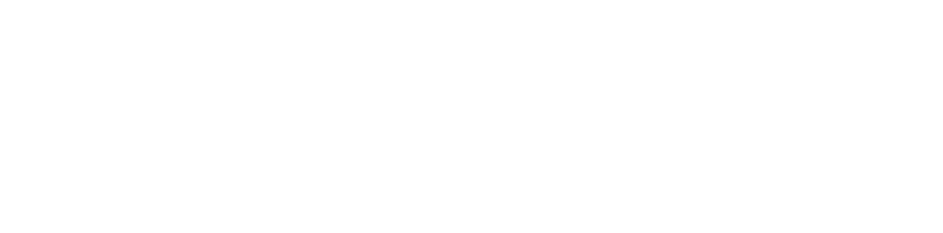
\includegraphics[scale=0.15]{../vlc.png}};
        \end{tikzpicture}
\end{frame}
}

\frame{
  \titlepage
}

\begin{frame}
\frametitle{Recap: Singular Value Decomposition and its applications}
Let's now change direction --- we're going to look at an early success story resulting from using some differentiation and the Singular Value Decomposition (SVD).
\\[1em]
For complex $\bm A:$ \\
\begin{align*}
\bm A &= \bm U \bm \Sigma \bm V^*
\end{align*}
where $\bm V^*$ is the \emph{conjugate transpose} of $\bm V$.\\[1em]
For real $\bm A:$ \\
\begin{align*}
\bm A &= \bm U \bm \Sigma \bm V^\top
\end{align*}
\end{frame}

\begin{frame}
\frametitle{Recap: Singular Value Decomposition and its applications}
\begin{itemize}
	\item SVD has many uses:
	\begin{itemize}
		\uncover<+->{
		\item Computing the Eigendecomposition:
		\begin{itemize}
			\item Eigenvectors of $\bm A\bm A^\top$ are columns of $\bm U$,
			\item Eigenvectors of $\bm A^\top\bm A$ are columns of $\bm V$,
			\item and the non-zero values of $\bm\Sigma$ are the square roots of the non-zero eigenvalues of both $\bm A\bm A^\top$ and $\bm A^\top\bm A$.
		\end{itemize}}
		\uncover<+->{
		\item Dimensionality reduction
		\begin{itemize}
			\item ...use to compute PCA
		\end{itemize}}
		\uncover<+->{
		\item Computing the Moore-Penrose Pseudoinverse
		\begin{itemize}
			\item for real $\bm A$: $\bm A^+ = \bm V \bm\Sigma^+ \bm U^\top$ where $\bm\Sigma^+$ is formed by taking the reciprocal of every non-zero diagonal element and transposing the result.
		\end{itemize}}
		\uncover<+->{
		\item<+-> Low-rank approximation and matrix completion
		\begin{itemize}
			\item if you take the $\rho$ columns of $\bm U$, and the $\rho$ rows of $\bm V^\top$ corresponding to the $\rho$ largest singular values, you can form the matrix $\bm A_\rho = \bm U_\rho \bm \Sigma_\rho \bm V^\top_\rho$ which will be the $best$ rank-$\rho$ approximation of the original $\bm A$ in terms of the Frobenius norm.
		\end{itemize}}
	\end{itemize}
\end{itemize}
\end{frame}

\begin{frame}
\frametitle{Example: Computing SVD using gradients - The Netflix Challenge}
\begin{itemize}
	\uncover<+->{\item There are many standard ways of computing the SVD:
	\begin{itemize}
		\item e.g. `Power iteration', or `Arnoldi iteration' or `Lanczos algorithm' coupled with the `Gram-Schmidt process' for orthonormalisation
	\end{itemize}}
	\uncover<+->{\item but, these don't necessarily scale up to really big problems
	\begin{itemize}
		\item e.g. computing the SVD of a sparse matrix with 17770 rows, 480189 columns and 100480507 non-zero entries!
		\item this corresponds to the data provided by Netflix when they launched the \emph{Netflix Challenge} in 2006. 
	\end{itemize}}
	\item<+-> OK, so what can you do?
	\begin{itemize}
		\item<+-> The `Simon Funk' solution: realise that there is a really simple (and quick) way to compute the SVD by following gradients...
	\end{itemize}
\end{itemize}
\end{frame}

\begin{frame}
\frametitle{Example: Computing SVD using gradients - The Netflix Challenge}
\framesubtitle{Deriving a gradient-descent solution to SVD}
\begin{itemize}
	\item<+-> One of the definitions of rank-$\rho$ SVD of a matrix $\bm A$ is that it minimises reconstruction error in terms of the Frobenius norm.
	\item<+-> Without loss of generality we can write SVD as a 2-matrix decomposition $\bm A = \hat{\bm U} \hat{\bm V}^T$ by rolling in the square roots of $\bm\Sigma$ to both $\hat{\bm U}$ and $\hat{\bm V}$: $\hat{\bm U} = \bm U \bm\Sigma^{0.5}$ and $\hat{\bm V}^\top = \bm \Sigma^{0.5} \bm V^\top$.
	\item<+-> Then we can define the decomposition as finding $\min\limits_{\hat{\bm U}, \hat{\bm V}}( \| \bm A - \hat{\bm U}\hat{\bm V}^\top \|_{\rm F}^2 )$
\end{itemize}
\end{frame}


\begin{frame}
\frametitle{Example: Computing SVD using gradients - The Netflix Challenge}
\framesubtitle{Deriving a gradient-descent solution to SVD}
\uncover<+->{
Start by expanding our optimisation problem:

\begin{align*}
	\min\limits_{\hat{\bm U}, \hat{\bm V}}( \| \bm A - \hat{\bm U}\hat{\bm V}^\top \|_{\rm F}^2 ) &= \min\limits_{\hat{\bm U}, \hat{\bm V}}( \sum_r \sum_c (A_{rc} - \hat{U}_r\hat{V}^\top_{:,c})^2 )	\\
			  &= \min\limits_{\hat{\bm U}, \hat{\bm V}}( \sum_r \sum_c (A_{rc} - \sum_{p=1}^{\rho}\hat{U}_{rp}\hat{V}_{cp})^2 )	 
\end{align*}
}

\uncover<+->{Let $e_{rc} = A_{rc} - \sum_{p=0}^{\rho}\hat{U}_{rp}\hat{V}_{cp}$ denote the error. Then, our problem becomes:

\begin{align*}
{\rm Minimise}\,\mathcal{L} &= \sum_r \sum_c e_{rc}^2
\end{align*}

We can then differentiate with respect to specific variables $\hat{U}_{rq}$ and $\hat{V}_{cq}$
}
\end{frame}


\begin{frame}
\frametitle{Example: Computing SVD using gradients - The Netflix Challenge}
\framesubtitle{Deriving a gradient-descent solution to SVD}
\uncover<+->{
We can then differentiate with respect to specific variables $\hat{U}_{rq}$ and $\hat{V}_{cq}$:
\begin{align*}
	\frac{\partial \mathcal{L}}{\partial \hat{U}_{rq}} &= \sum_r \sum_c 2e_{rc} \frac{\partial e}{\partial \hat{U}_{rq}} = -2 \sum_r \sum_c \hat{V}_{cq} e_{rc} \\
	\frac{\partial \mathcal{L}}{\partial \hat{V}_{cq}} &= \sum_r \sum_c 2e_{rc} \frac{\partial e}{\partial \hat{V}_{cq}} = -2 \sum_r \sum_c \hat{U}_{rq} e_{rc} \\
\end{align*}
}

\uncover<+->{
and use this as the basis for a gradient descent algorithm:

\begin{align*}
	\hat{U}_{rq} &\Leftarrow \hat{U}_{rq} + \lambda \sum_r \sum_c \hat{V}_{cq}e_{rc} \\
	\hat{V}_{cq} &\Leftarrow \hat{V}_{cq} + \lambda \sum_r \sum_c \hat{U}_{rq}e_{rc}
\end{align*}
}

\end{frame}

\begin{frame}
\frametitle{Example: Computing SVD using gradients - The Netflix Challenge}
\framesubtitle{Deriving a gradient-descent solution to SVD}

\begin{itemize}
	\item<+-> A stochastic version of this algorithm (updates on one single item of $\bm A$ at a time) helped win the Netflix Challenge competition in 2009.
	\item<+-> It was both \emph{fast} and \emph{memory efficient}
\end{itemize}

\end{frame}

\end{document}